% Created with jtex v.1.0.20
\documentclass{article}
\PassOptionsToPackage{short, nodayofweek}{datetime}

\input{curvenote.def}



% colors for hyperlinks
\hypersetup{colorlinks=true, allcolors=blue}
\hypersetup{
pdftitle={\@title},
pdfsubject={description},
pdfauthor={\@author},
pdfkeywords={},
addtopdfcreator={Written in Curvenote}
}

\usepackage{curvenote}

\title{CT scan reconstruction using machine learning}

\newdate{articleDate}{1}{1}{2024}
\date{\displaydate{articleDate}}

\author{\bfseries Luuk Fröling\mdseries\\}

\begin{document}

\maketitle

\textbf{Author:} Luuk Fröling

\section{abstract}

abstract, work in progress

\section{Introduction}

With the invention of the first viable CT scanner in 1972 by Godfrey Hounsfield, funded in part by sales from `the beatles' records \citep{pietzsch2025ct}, the field of medical imaging gained the ability to produce cross-sectional images of a human body. In computed tomography (CT), these images are generated by rotating both an x-ray source and a detector around the object being scanned. The resulting images show, like regular x-ray images, how much radiation is absorbed per voxel (the attenuation coefficient). However, different materials may exhibit similar absorption properties, making it difficult to distinguish between them in conventional CT scans.

With the introduction of photon counting detectors (PCD), which can detect individual photons and their energy \citep{taguchi2013photon}, the energy dependence of the attenuation coefficient of a material can be utilised to differentiate materials that appear identical on x-rays acquired using energy integrating detectors (EID). By sorting the detected photons into energy bins, multiple measurement spectra can be generated to reconstruct an images displaying the distributions of different materials.

This technique, known as material decomposition, requires advanced reconstruction algorithms. These algorithms, like an iterative algorithm proposed by \citep{mechlem2018joint}, are often computationally heavy and time-consuming. If successfully implemented, dual-energy CT scan images provide in-depth information about the types of tissue present in an image.

Recent advances in machine learning and neural networks, particularly U-Nets \citep{oktay2018attentionunet} and attention mechanisms  \citep{vaswani2017attention}, have shown great potential for image reconstruction tasks. Combining these techniques can allow a model to be capable of learning complex spatial relationships, where such model has the potential to accelerate or even replace traditional iterative methods.

In this work, an attention-based U-Net (AttU-Net) is employed to replace the steps of the iterative reconstruction algorithm. The input data consists of projections acquired using a PCD, which provides energy-dependent measurements by sorting the measured photon counts in energy-bins. Focusing on the material decomposition capabilities of dual-energy CT scans, the AttU-Net model is trained to iteratively reconstruct both water and bone density images based on training data taken from the iterative reconstruction algorithm described in \citep{mechlem2018joint}.
// Should I add this? to above paragraph? To assess the model's performance, both quantitative and qualitative evaluation methods are applied, including error metrics and visual comparisons.

For training, simulated projection data is generated using phantoms consisting of a cylindrical body with two distinct regions: one with higher bone density and one with higher water density. After training the model on these phantoms, validation is performed using a separate set of 20 unseen phantoms. The reconstructed images are evaluated using root-mean-squared (RMS) error analysis and visual inspection. Additionally, a speedup metric is introduced to compare how quickly the AttU-Net reaches a comparable RMS error to that of the iterative method.

\section{Theory}

\subsection{Basics CT scans}

A computed tomography (CT) scanner is an imaging device that uses x-rays to create cross-sectional images of an object. It consists of an x-ray source and a detector placed at a distance from each other. During scanning, both the source and the detector will rotate around the object to be imaged at several angles. For each step, the source emits x-rays that pass through the object; the transmitted photons are measured by the detector. The number of detected photons at position i along the detector is given by:

\begin{equation}
\label{first }
\hat{y}_i  = N_0 \cdot \exp\left(-\int \mu(x, E) \, dx\right)
\end{equation}

where $N_0$ is the number of the x-rays emitted by the source, $\mu(x, E)$ is the linear attenuation coefficient and the integral in the exponent represents the cumulative attenuation along the x-ray path. $\mu(x, E)$ describes how many of the incoming x-rays are absorbed per unit of length, which depends on both the material of the object and the energy of the x-ray $E$ \citep{kamalian2016ct_principles}.

By rotating the source and detector around the object and recording measurements at multiple angles, a sinogram can be created. A sinogram is a 2D plot where each row corresponds to a detector reading at a specific projection angle.

\begin{figure}[!htbp]
\centering
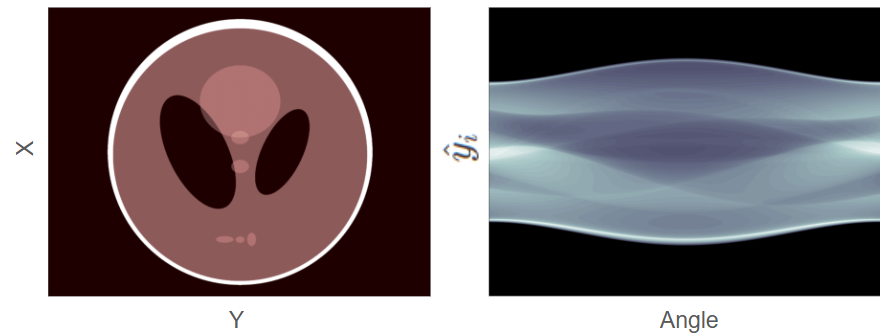
\includegraphics[width=0.7\linewidth]{files/sinogram2-4fe5b9d9d15b3f851681be6aafbc4af0.png}
\caption[]{\textit{left:} A phantom with multiple structures (ellipses) of different densities  \textit{right} corresponding sinogram. The darker regions in the sinogram indicate higher photon counts. \textit{Figure reproduced from} \citep{leuschner2019lodopab}}
\label{phantomSinogram}
\end{figure}

A phantom and a corresponding sinogram can be seen in Figure~\ref{phantomSinogram}. The phantom contains multiple, elliptical structures of different densities. On the right is the corresponding sinogram where the darker parts of the sinogram correspond to more detected photons.

\subsection{Cone beam CT scan}

The sinogram in Figure~\ref{phantomSinogram} is true for a 1D detector, where we construct a single slice. A cone beam CT scan uses a source emitting x-rays in a cone-beam shape, which can be detected on a 2D flat-panel detector \citep{venkatesh2017cbct}.

\begin{figure}[!htbp]
\centering
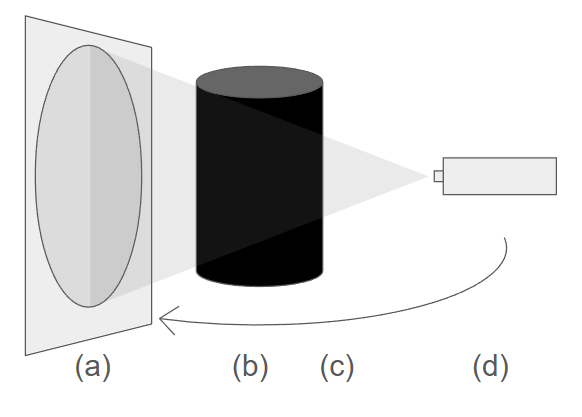
\includegraphics[width=0.5\linewidth]{files/cone_beam_ct-99b3680584828e6b48ebd5424f1fe103.png}
\caption[]{A schematic drawing of a cone-beam CT scan: (a) the 2D detector panel, (b) the phantom, (c) rotation direction of the source-detector pair (d) the x-ray source.}
\label{cone_beam}
\end{figure}

Figure~\ref{cone_beam} shows a cone beam CT scan setup, where both the detector and the source rotate around the object to acquire a set of 2D projection images at multiple angles. these measurements are known as projections and allow for a 3D image to be reconstructed.

The relationship between the object and the measured rays can be described by a projection matrix $A$. This matrix has dimensions $M \times N$ where $N$ is the number of voxels in the object and $M$ is the number of rays (measurements) collected by the detector. Each element $a_{mn}$ of the matrix is the contribution of the nth voxel of the object to be imaged to the mth ray of the detector \citep{Yang2017ProjectionMatrix}. The measured projections can thus be modeled as:

\begin{equation}
\label{projection_eq}
y = Ax
\end{equation}

where $x$ is the vectorised representation of the voxel values and $y$ contains the corresponding ray measurements. This formulation will be used by the reconstruction algorithms during the simulations. To better reflect the statistical fluctuations during photon detection, noise is applied to the computed projections. Measured counts are drawn from a poisson distribution with a mean equal to the ideal (noise-free) projection values as described by equation (\ref{projection_eq}).

\subsection{Detector types}

Currently, most CT scanners use an energy integrating detector (EID) \citep{marth2023photon}. An EID measures the intensity of the incoming x-rays by a two-step process: scintillation followed by photodetection. The scintillator absorbs the x-rays which have passed through the body and emits light in the visible spectrum. These re-emitted photons can be detected by photodetectors located underneath the scintillator. Due to the difference in energy of the incoming x-ray and the emitted visible light, multiple light photons can be re-emitted. To measure a signal, EIDs integrate over time which loses all energy dependent information \citep{taguchi2013photon}.

\begin{figure}[!htbp]
\centering
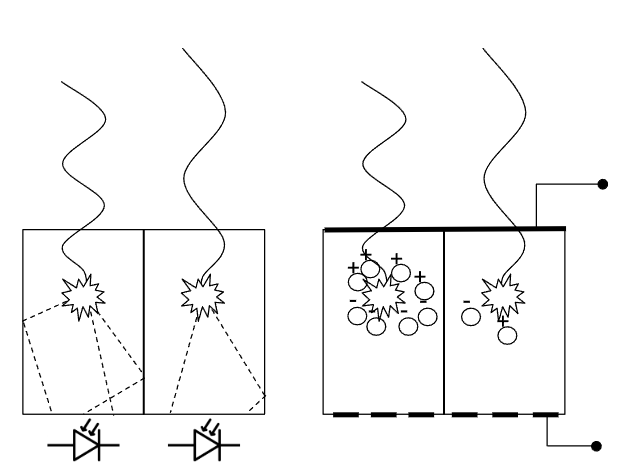
\includegraphics[width=0.5\linewidth]{files/detectorTypes-1f23300987a3b96a7f3effc6cb05b528.png}
\caption[]{\textit{left:} An EID where the incoming x-rays are absorbed within the scintillator. Several photons within the visible light spectrum are re-emitted which can be measured by the photodiodes located below the scintillator. \textit{right:} A PCD where incoming x-rays create electron-hole pairs in a semiconductor. This creates a current between the top and bottom of the semiconductor which can be measured by electrodes, preserving energy dependent information.}
\label{detectors}
\end{figure}

Photon-counting detector (PCD) CT scans improve the measurements by directly transforming the incoming X-ray photons into an energy-dependent signal, as illustrated in Figure~\ref{detectors}. In a PCD, each photon is absorbed in a semiconductor layer, generating electron-hole pairs that produce an electric signal proportional to the photon's energy. Unlike EIDs, PCDs can measure the energy of individual photons.

Commonly available X-ray sources emit a polychromatic spectrum \citep{Antsiferov2003}, meaning the emitted photons span a broad range of energies rather than a single energy level. The PCD measures the energy of the incoming photons and sorts these into multiple energy bins, each representing a specific range within the spectrum \citep{pcd2022}. By comparing the counts across these energy bins, multiple energy-resolved measurements can be done.

\subsection{Material decomposition}

Since different materials attenuate x-rays differently across the energy spectrum, PCD-CT can be used to distinguish between different tissue types in the body. To simulate this process and to describe the attenuation properties of different materials in a phantom, material decomposition is used \citep{mechlem2018joint}. In clinical practice, human tissue can be approximated as a linear combination of two basis materials, commonly water and bone, which simplifies the decomposition process.

\begin{figure}[!htbp]
\centering
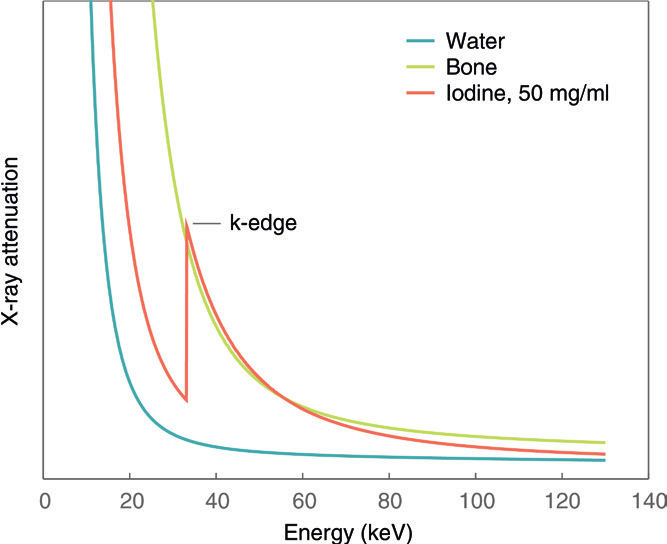
\includegraphics[width=0.7\linewidth]{files/att_map-6b5577988a8a3212ab72b98e5006371b.png}
\caption[]{The linear attenuation coefficient ($\mu$) of bone (green), water (blue) and iodine (orange) plotted as a function of the incoming X-ray photon energy. Iodine exhibits a k-edge, characterised by a sharp increase in attenuation at a specific energy, making it unsuitable be modelled as a linear combination of bone and water. \textit{Figure reproduced from} \citep{Willemink2018PhotonCountingCT}}
\label{matatt}
\end{figure}

The linear attenuation coefficient ($\mu$), which describes how a material attenuates X-rays, depends on both the material and the photon energy, as shown by the attenuation curves in Figure~\ref{matatt}. For bone, water and other forms of tissue in the human body these attenuation curves can be assumed smooth within the energy range used \citep{Willemink2018PhotonCountingCT}.  However, contrast agents such as iodine display one or more K-edges, sudden increases in attenuation at specific energies, which cannot be accurately modeled by a simple combination of water and bone. In this work, only bone and water will be used. If a contrast agent were to be involved, a 3rd material must be added to compensate for any possible k-edges.

In this work the reconstructed image of the PCD CT scan will therefore consist of 2 images. One displaying the bone density and one displaying water density. The linear attenuation coëfficient of any material within the phantom can then be described as:

\begin{equation}
\label{muE}
\mu(E) = \sum_{b=1}^{B} A_b f_b(E)
\end{equation}
where $A_b$ is the line integral of material b, representing the amount of material b in the beam path, and $f^b(E)$ describes the attenuation coefficient of the basis material b. Combining equation (\ref{first}) and (\ref{muE}) gives an expression for the photon count at the detector:

\begin{equation}
\hat{y}_i = \int_0^{\infty} \phi_{\text{eff},i}(E) \exp\left( - \sum_{b=1}^{B} A_b^i f_b(E) \right) \, dE
\end{equation}

where $\phi_{\text{eff},i}(E)$ represents the effictive x-ray spectrum which includes both the shape of the X-ray source spectrum and how the detector responds to photons of different energies. The detector does not detect all photon energies equally well, some energies are absorbed more efficiently than others or may be missed due to noise or other effects.

\subsection{Projection algorithms}

To view the cross-sectional image of an object from these measurements, either from a detector or from simulations using equation (\ref{projection_eq}), a reconstruction algorithm needs to be used. Filtered back projection (FBP) is an analytical reconstruction algorithm; during reconstruction, each projection is spread back across the image plane along the same angle it was acquired. This often leads to blurry images as the intensity is spread along lines rather than concentrated at specific points \citep{zeng2001image}. A filter is used to help sharpen the image and reduce blurring artifacts. FBP can be used for spectral-CT scans by a two-step image based method. The first step is to reconstruct an image for each energy bin and these intermediate images are then decomposed into material-dependent images \citep{mory2018comparison}.

The two-step, image based method has several drawbacks. First, beam hardening artifacts often occur as the attenuation coefficient is still averaged over a line. Secondly, the first step leads to a loss of information as there is no one-to-one mapping between the projections and the images. The second step is unable to compensate for this loss as it has no access to the photon counts. Recently one-step methods have been proposed which reconstruct material-specific images directly from photon counts \citep{mechlem2018joint}. These are all iterative methods as no analytical inversion formula exists.

An iterative reconstruction algorithm starts with an initial guess of the image and, at each iteration updates the image to better match the measured data. This is done according to a cost function, which depends on how well the image assumption explains the measured photon counts (data fidelity term), and how smooth, or physically plausible the images is (regularization term) \citep{Zhang2018Regularization}. The iterative algorithm used, uses a seperable quadratic surrogates (SQS) cost function.

\begin{figure}[!htbp]
\centering
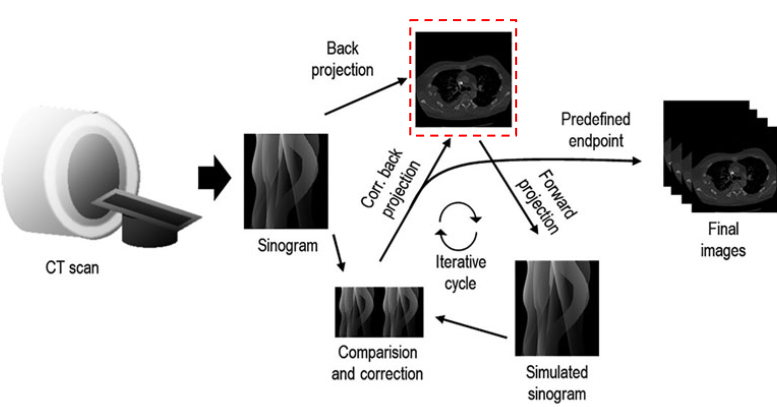
\includegraphics[width=0.7\linewidth]{files/itt-034b6f212be5f30f95f77cb82041b170.png}
\caption[]{An overview of an iterative reconstruction algorithm. From the measured projections a reconstructed image is estimated. This image is then iteratively compared with the original sinogram in the forward projection and corrected until a predefined endpoint. This work makes use of 40 iterations as an endpoint. \textit{Figure reproduced from} \citep{arndt2021deeplearning}}
\label{itt}
\end{figure}

A downside to the iterative algorithm is the computational time. For each iteration there is a forward projection and a backprojection, as well as an error calculation. There is also a large amount of iterations needed to get to an accurate solution. This work will look at including machine learning to replace the iterative steps.

\subsection{Machine learning - Neural networks}

Neural networks are a subset of machine learning and play a crucial role in deep learning algorithms. A simple, fully connected neural network consists of nodes stacked in layers: an input layer, one or more hidden layers and an output layer.

\begin{figure}[!htbp]
\centering
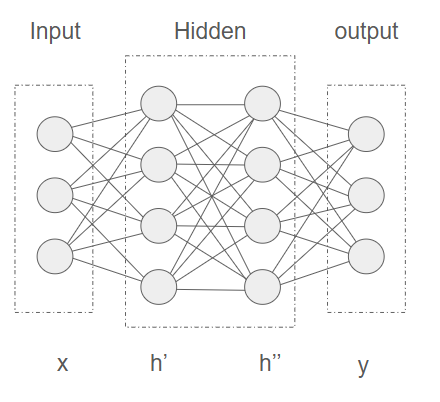
\includegraphics[width=0.7\linewidth]{files/neuralnetwork-7c664ffdc7b4a7b98a97346c5a4ef4fb.png}
\caption[]{A neural network consisting of 3 input nodes, 2 hidden layers with 4 nodes each and an output layer with 3 nodes. The input values are represented by an array x, the hidden layers by array h' and h'' and the output layer by y.}
\label{neural_network}
\end{figure}

All nodes in a layer are connected to an adjacent layer by weigths. Figure~\ref{neural_network} shows a simple neural network, where input layer x and first hidden layer h' are connected by a matrix of weights $W_1$, the states of the first hidden layer can be calculated as

\begin{equation}
\label{denseLayer}
\mathbf{h}_1 = \sigma(\mathbf{W}_1 \mathbf{x} + \mathbf{b}_1)
\end{equation}
with $\mathbf{W}_{1,nm}$ representing the weight connecting the m-th input neuron to the n-th neuron in the first hidden layer, and $\sigma$ is an activation function (e.g., sigmoid or softmax) that scales the output between 0 and 1 to stabilise the network and to introduce non-linearity. Equation (\ref{denselayer}) can be repeated for every following layer where the output of a layer is used as an input to calculate the following layer.

Neural networks are generally trained using the backpropagation algorithm, which relies on a dataset consisting of input-output pairs. During training, the network processes each input and generates an output, A cost function determines the error between the network's output and the target output. This cost function guides the learning process by indicating how far the network's predictions are from the desired outputs. The backpropagation algorithm will look at how each weigth in the network needs to change to minimalise the error.

\subsection{Machine learning - Convolutional neural network}

A convolutional neural network (CNN) can be used to more accurately extract features from images for processing, where a feature is a characteristic or pattern in the input data. A CNN consist of a kernel (also called a filter) and one or more channels. The kernel is smaller than the input data but has the same number of dimensions (e.g., 2D for 2D images). The kernel contains weights that are learned during training.

The kernel is moved across the input data, performing element-wise multiplication with the region of the input it covers, followed by a sum. This operation extract features such as edges, textures and shapes \citep{yamashita2018convolutional}. We can write the output feature map of a convolutional layer as

\begin{equation}
S(i, j) = (\mathbf{K} * \mathbf{X})(i, j) = \sum_m \sum_n \mathbf{K}(m, n) \cdot \mathbf{X}(i + m, j + n)
\end{equation}

where $(i,j)$ are spatial indices, $\mathbf{X}$ the relevant kernel and $(m,n)$ the kernel indices. After a convolution layer, $S(i, j)$ can be either vectorised to be used as an input for a fully connected layer as described in equation (\ref{denseLayer}) or used as an input for a second convolution layer. Due to a kernel only working on adjecent pixels, convolutional layers extract local features.

\begin{figure}[!htbp]
\centering
\begin{verbatim}
Text(0, 0.5, 'Y')
\end{verbatim}

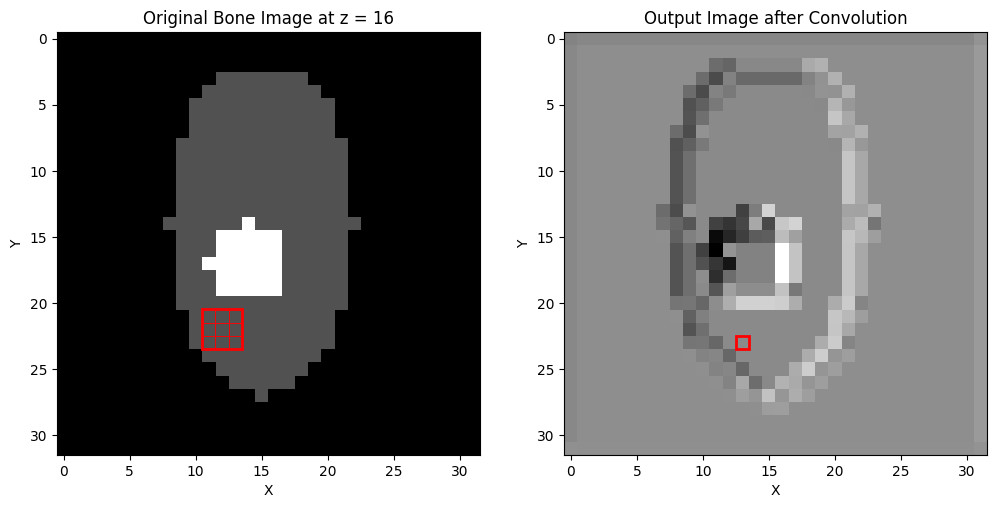
\includegraphics[width=0.7\linewidth]{files/df9eecf15dc213c5837add0b2c07a681.png}
\caption[]{\textit{left :} original phantom with a 2D 3x3 randomly initialised kernel drawn on top. each individual square represents a pixel, with the outer square representing the kernel. \textit{right :} phantom after 2D convolution layer has been applied.}
\label{convex}
\end{figure}

The left part of Figure~\ref{convex} shows a 3x3 convolution kernel with randomly initialised weights (red) placed on a phantom and the right part of the figure shows the imgage of the phantom after the convolution. Even with randomly initialised weights, there is already an edge-detection like pattern. The image on the right is called a feature map, as each pixel represents higher-level information of the original image.

A CNN typically consists of multiple layers stacked on top of each other, allowing deeper feature extraction. Early layers can detect simple features like edges, while deeper layers can detect more complex structures like shapes and objects.

\subsection{Machine learning - U-Net architecture}

Multiple convolution layers can be combined to form an encoder. An encoder generates an abstract representation of an input image by repeatedly performing convolution and progressivly reducing the size of the image. This reduction is achieved using max pooling layers, which divide the input into rectangular regions and takes the maximum value from each region, reducing the image size and allowing the network to capture more abstract and higher-level data between layers.

Similarly a decoder can be used generate an output image from the abstract representation. A decoder uses deconvolution layers which progressively increases the size of the image, adding features back in at each step to refine the output.

\begin{figure}[!htbp]
\centering
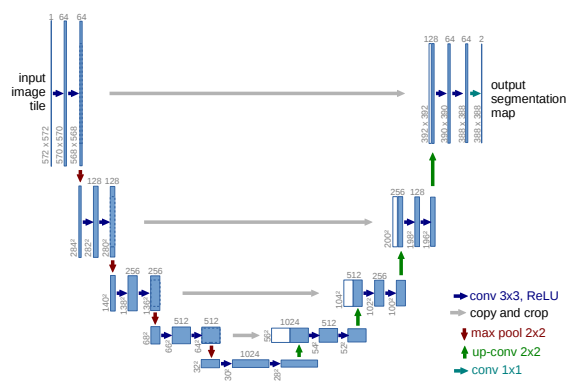
\includegraphics[width=0.75\linewidth]{files/Unet-b453ddb3b21672f27228e873588d59c4.png}
\caption[]{A U-Net architecture for an image with a 32x32 lowest possible resolution. Each blue square represents a multi-channel feature map with the amount of channels denoted on top of the box. Gray arrows represent cross over layers with the white boxes representing copied layers from the encoder \textit{Figure reproduced from} \citep{oktay2018attention}}
\label{unet}
\end{figure}

By combining an encoder and a decoder, a U-Net can be constructed as illustrated in Figure~\ref{unet}. Between each layer of the encoder and decoder part of the network, there is a skip-connection layer which copies the feature map from the encoder layer to the decoder layer. This allows the decoder to use features during reconstruction which might have been lost while encoding the image.

\subsection{Machine learning - Attention gate}

For feature extraction from images where both local and non-local features are of importance, convolution layers can be combined with attention mechanisms. An attention mechanism allows machine learning models to attend to the most relevant parts of the input data \citep{vaswani2017attention}.

An attention mechanism takes the input vector $x_{i}^{l}$ and multiplies it by an attention score $\alpha_{i}^{l}$ to preserve only the activations relevant to the task. To calculate $\alpha_{i}^{l}$,  an intermediate attention score $q_{\text{att}}^{l}$ (the attention score $q_{\text{att}}$ for layer l) can be defined as
\begin{equation}
q_{\text{att}}^l(x_i^l, g_i) = \psi^{T} \, \sigma \left( W_{x}^{T} x_{i}^{l} + W_{g}^{T} g_{i} + b_{g} \right) + b_{\psi}
\end{equation}
where $g_{i}$ the gating feature vector, $W_{x}^{T}$ and $W_{g}^{T}$ weight matrices similar to those used in equation (\ref{denseLayer}), $\psi^{T}$ another learned linear transformation and $\sigma$ an activation function. The gating feature vector provides contextual information from higher-level layers. It acts as a control signal that guides the attention mechanism, helping it decide which parts of the input to focus on. The final attention coefficient $\alpha_{i}^{l}$, the final attention mask that says which parts of the feature map should be passed forward, is then calculated as

\begin{equation}
\alpha_{i}^{l} = \sigma \left( q_{\text{att}}^{l}(x_{i}^{l}, g_{i}; \Theta_{\text{att}}) \right)
\end{equation}
with $\Theta_{\text{att}}$ representing the learned parameters of the attention block: all weights and biases. The final output of the attention gate is

\begin{equation}
\tilde{x}_i^l = \alpha_i^l \cdot x_i^l
\end{equation}

where regions get $\alpha = 1$ where less important regions get $\alpha \approx 0$

\begin{figure}[!htbp]
\centering
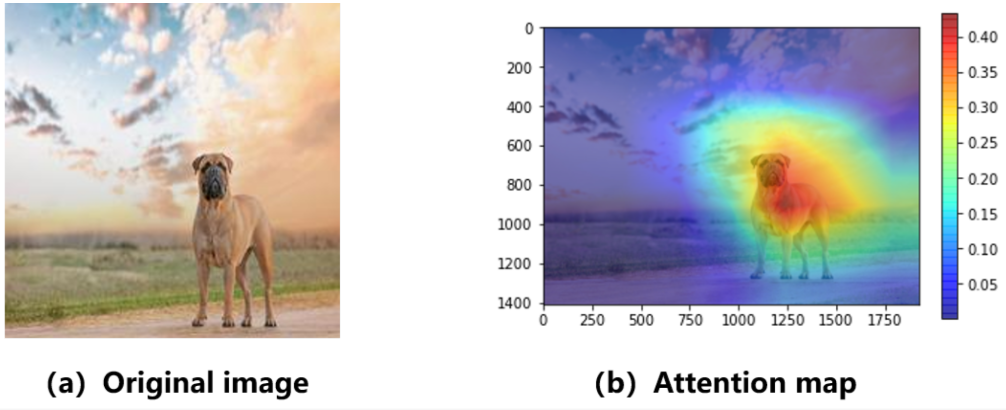
\includegraphics[width=0.7\linewidth]{files/dog-90a3cc53b4e9c683fe6e5d12d3707cd0.png}
\caption[]{Example image from an attention-based network trained to label images. Image a shows a picture of a dog which the network needs to label and image b shows the attention map which is the value of $\alpha$ per pixel.  \textit{Figure reproduced from} \citep{An2022Attention}}
\label{dog}
\end{figure}

An example has been taken from \citep{An2022Attention}, where an attention-based network has been trained to label images. An input image can be seen on the left in Figure~\ref{dog} where the label is supposed to be `dog'. A heatmap for the value of $\alpha$ is shown on the right where we can see the attention mechanism provides a strong focus on the part of the image where the dog is located.

\subsection{Machine learning - Attention U-Net}

Attention mechanisms can be added to the skip-connections of the U-Net model in Figure~\ref{unet}, allowing the network to focus on non-local features during the reconstruction of the image. The combination of attention mechanism and convolutional layers can be used to recognise certain features like edges and to make connection between features in different parts of the image \citep{oktay2018attentionunet}.

\begin{figure}[!htbp]
\centering
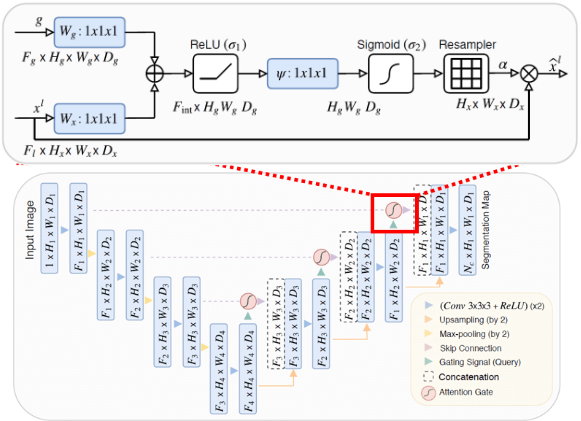
\includegraphics[width=0.7\linewidth]{files/AttU-Net-86c6f656da029e6df27f6848620cbcbe.png}
\caption[]{Schematic overview of a U-Net model with attention gates added to the skip-connections. The inset (top) shows a zoomed-in view of an attention gate, the gating signal $g$ is taken from the previous decoding layer and the input $x^l$ is the skip-connection layer. \textit{Figure reproduced from} \citep{oktay2018attentionunet}}
\label{attunet}
\end{figure}

The attention gate uses the gating signal $g$ to modulate the features passed through the skip connection. This mechanism allows the network to selectively emphasize relevant spatial features and suppress irrelevant or noisy information. Each skip connection uses the output of the previous decoder layer as a gating signal to control which encoder features are passed forward, as illustrated in Figure~\ref{attunet}.

\section{Method}

\subsection{Overview}

A machine learning model will be trained to use information from sinogram space to adjust images in image space. The network will be trained to perform this conversion in iterative steps similar to the iterative reconstruction method described in \citep{mechlem2018joint}.

\begin{figure}[!htbp]
\centering
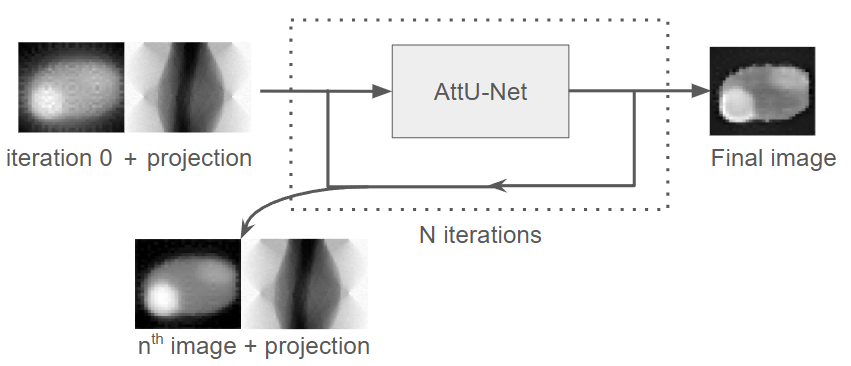
\includegraphics[width=0.7\linewidth]{files/model2-ec3da612d514bb3090ae242dc099057b.png}
\caption[]{Schematic overview of the model workflow. The input to the model consists of the initial reconstructed image from iteration 0 combined with the corresponding projection (sinogram) data. The network processes this input iteratively, where the output of the $n^{th}$ iteration is used as the input for the $(n+1)^{th}$ iteration, while the projection data remains constant. After N iterations, the final reconstructed image is produced.}
\label{model2}
\end{figure}

An overview of the model workflow is shown in Figure~\ref{model2}. The network is designed to use the first reconstructed image from the iterative algorithm (called iteration 0 for the AttU-Net model) combined with the projection matrix and refine the reconstructed image across 40 iterations. The output image of an iteration is used as an input for the following iteration, making sure the projection matrix remains constant. After 40 iterations, the output of the network is used as the final image.

\subsection{Generating phantoms}

The training data consists of phantoms generated according to a set of rules for which projections are simulated. These projections are used by the iterative algorithm, where the intermediate images are used as training data for the model. The phantoms are randomly generated according to a set of rules:

\begin{itemize}
\item each phantom is 32x32x32 pixels and consists of 2 channels, one for bone and one for water.
\item each phantom has a main, elliptical body centered in the image consisting of a low mass density of both water and bone (both densities uniformly distributed between 0.1 and 0.6).
\item The center of the body can be randomly offset by -3 to +3 pixels in both the x and y directions (uniform distribution).
\item The size of the main body varies, with the distance between the points on the axis varying between 1 and 3 pixels uniformly distributed.
\item Each phantom has 2 internal features, represented as smaller elliptical regions within the main body.
\item Each feature has either a higher bone density or a higher water density than the other.
\item The bone and/or water density cannot be lower in a feature than the main body
\end{itemize}

Each feature represents a distinct elliptical region. Because photon counting detectors (PCDs) allow differentiating tissue types, we assign one feature a higher bone density and the other a higher water density. This design ensures that the network is trained on a task relevant to the clinical use of PCDs. These rules have been implemented in python to generate a sample of phantoms as seen in the supporting notebooks.

\subsection{Acquiring data}

For 506 phantoms, detector measurements are simulated. These measurements are done with 32 angles per phantom. Next, each set of detector measurements are reconstructed using the iterative algorithm with 40 iterations. These iterations are used to construct input-output pairs for training the model. Using a stride (how many images to skip between input and output images), the input is defined as the image from the $n^{th}$ iteration, with a corresponding output image taken from the $(n+stride)^{th}$ iteration.

Using a stride between input and output images allows the model to learn from a wider variety of scenarios within the same training time. In this work, a stride of 4 is used. This work made use of 506 phantoms, which generated 4554 input-output pairs.

\subsection{Attention based U-Net}

To enable the network to learn how features in the image space and the projection (sinogram) space attend to eachother, a U-Net architecture with attention mechanisms integrated into the skip connections is used (AttU-Net) as described by \citep{oktay2018attentionunet}. The attention gates help the model to focus on which parts of the sinogram contribute to specific image regions.

The AttU-Net model is illustrated in Figure~\ref{attunet}. The architecture consists of five convolutional encoder blocks, a bottleneck block, and five decoder blocks. The number of channels increases through the encoder (64, 128, 256, 512 and 1024), and then decreases symmetrically through the decoder. The output layer applies a sigmoid activation to produce voxel-wise probabilities. The model has been implemented in Python using Pytorch in the supporting notebooks

The model is trained on an NVDIA Tesla A100, with 4 hours allocated per run. In total 6 runs were completed, which resulted in 180 epochs (20 epochs per run). The model uses MSELoss as a loss function and Adam optimisation, which is a stochastic gradient descent method. The learning rate is set to 0.001, which is commonly used with Adam optimisation \citep{kingma2014adam}. An implementation of the training function can be seen in the supporting notebooks

\subsection{Shaping the data}

The AttU-Net model takes an image as input and produces an image of the same size as an output. Since 2 different images are used (the image and the projection), these must be combined into a single matrix. The projection matrix has dimensions (number of projections) x (z pixels detector) x (y pixels detector), where this work uses 32 projections and a detector of 64 by 44 pixels as set for the simulations in the supporting notebooks.

Aditionally, due to the pooling layers all dimensions must be powers of 16 as to not get an uneven amount of devisions. The projection matrix is originally 32 x 44 x 64 pixels, which we can pad with zeros to 32 x 48 x 64 pixels. The image will is 32 x 32 x 32 pixels which we can pad to 32 x 48 x 32 to fit the dimensions of the projections. The final input set to the network will be 10 x 32 x 48 x 96 as we use 10 channels in total.

\subsection{Validation}

20 phantoms have been used as a validation set, generated under the same conditions and rules as those used for training. The performance of both the AttU-Net model and the iterative algorithm will be compared by calculating the root-mean-square (RMS) error between a reconstructed image and the GT image. The RMS error is calculated as

\begin{equation}
\text{RMS\_error} = \sqrt{ \frac{1}{N} \sum_{i=1}^{N} \left( I_1(i) - I_2(i) \right)^2 }
\end{equation}

where $I_1(i)$ and $I_2(i)$ are the pixel values at position $i$ in image 1 and image 2, respectively. N is the total number of pixels in the image, 32768 pixels in this case.

\section{results}

\subsection{Visualisation reconstruction}

During evaluation the model has been run on 20 validation sets generated under the same conditions and rules as those used for training. By taking the first image from the iterative algorithm, 20 reconstructions can be made using the proposed AttU-Net model.

\begin{figure}[!htbp]
\centering
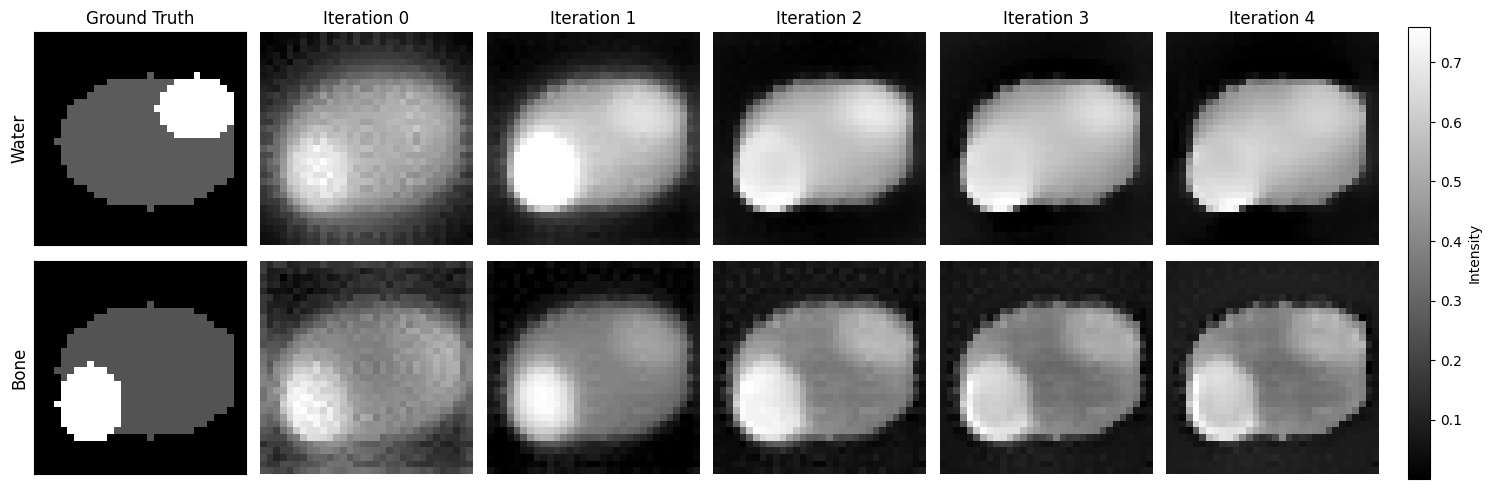
\includegraphics[width=0.7\linewidth]{files/7919280d54a67f0898be36384abd7990.png}
\caption[]{Top row (water), left to right: Ground truth (GT) water image; iteration 0 (first reconstruction) from iterative algorithm; subsequent reconstructions by the model.
Bottom row (bone), left to right: GT bone image; iteration 0 (first reconstruction) from iterative algorithm; subsequent reconstructions by the model.}
\label{bone_recons}
\end{figure}

The first 4 reconstructions of the second phantom are displayed in Figure~\ref{bone_recons} and the first column displays the ground truth (GT) images as a reference. The rows show the reconstruction process using the model for water and bone respectively, where each column is an iteration. In the GT images, distinct features are visible: a bone structure in the lower left quadrant and a water structure in the top right quadrant. These serve as reference to evaluate the reconstruction quality.

The first reconstruction shows that the AttU-net model accurately recongnises the key features of the phantom, however the water feature is faint in the water density image. As reconstruction progresses, the overall water density increases while the edges between distinct features of the phantom are blurred. The bone density image looks to converge to a state where the phantom's body has a lower density, with both water and bone features present.

\subsection{Visualisation comparison}

To better understand the quality of the images compared to the iterative algorithm, the iterative algorithm has been used to reconstruct the phantoms as well using the same parameters as used during training.

\begin{figure}[!htbp]
\centering
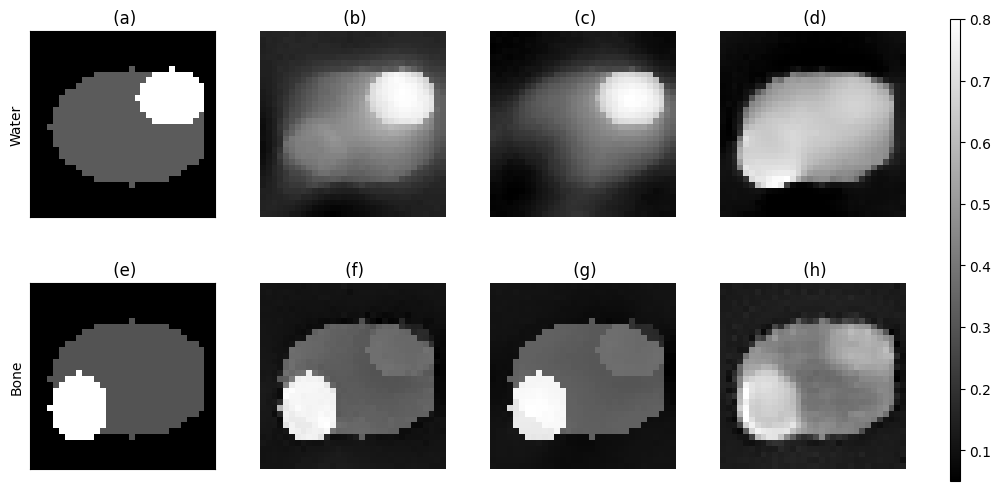
\includegraphics[width=0.7\linewidth]{files/afec7fb8a942be43385875429673a4f0.png}
\caption[]{(a) GT water image (b) smallest RMS water image iterative algorithm (c) water image from last iteration iterative algorithm (d) water image reconstructed by the model after 3 iterations (e) GT bone image (f) smallest RMS bone image iterative algorithm (g) bone image from last iteration iterative algorithm (h) bone image recontructed by the model after 3 iterations.}
\label{reconPhantom}
\end{figure}

Looking at the reconstructions corresponding to the smallest root mean square (RMS) error across all iterations (panel b and f), both water and bone features are present in their respective images. However the iterative algorithm does not fully distinguish between the materials of the two features, as the water feature can be faintly seen in the bone images and vice versa. For the final iteration of the iterative algorithm (panel c and g), the water image shows a clear reduction of the bone feature. This indicates an overcompensation compared to panel b.

Eventough more blurry, the bone image reconstructed by the AttU-Net model has the same level of pattern recognition as the iterative algorithm. The model was unable to recognise these features in the image for water, while the iterative algorithm does. The images generated by the model also have a lower contrast between features compared to the iterative approach.

\subsection{RMS over time}

By calculating the RMS error at each iteration for both the iterative algorithm and the model with the ground truth (GT) image, we can compare the reconstruction errors as a function of time.

\begin{figure}[!htbp]
\centering
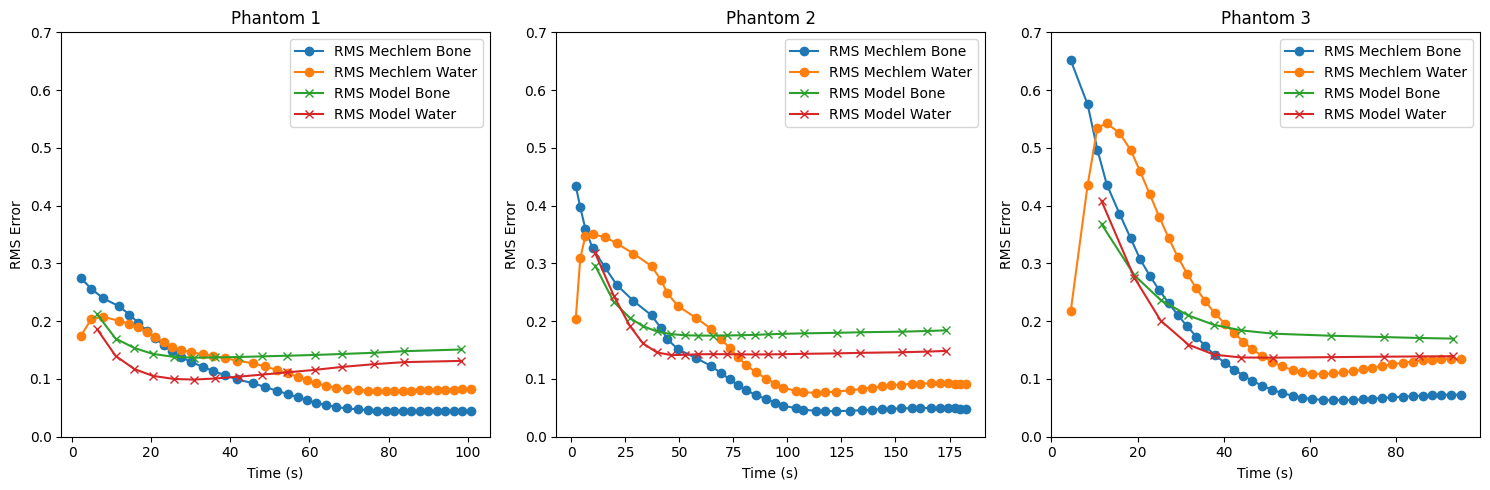
\includegraphics[width=0.7\linewidth]{files/586fa19a8938bf6fcb255a7e08c69611.png}
\caption[]{RMS error over time for three phantoms reconstructed using both the iterative method (orange: water; blue: bone) and the proposed AttU-Net model (red: water; green: bone).}
\label{rmsTime}
\end{figure}

Figure~\ref{rmsTime} shows the RMS error over time for bone and water images reconstructed by both methods for the first 3 phantoms from the validation set, where the second phantom can be seen in Figure~\ref{bone_recons} and Figure~\ref{reconPhantom}. The AttU-Net model has been run for as long as it took for the iterative algorithm to complete all 40 iterations. In all three cases, the model achieves a lower initial error but converges to a larger error compared to the iterative algorithm. For both algorithms the RMS error of the water images converges to a higher value than the RMS of the bone images.

Looking at a dataset of 20 phantoms, the average time taken for the first iteration of the model is 9.3 seconds with a standard deviation of 1.5 seconds. The average speedup for bone for this step is 1.44 times, or 44\% while the average speedup for water is 1.17 times, or 17\%. The speedup is defined as the time it takes for the iterative aproach to reach the same RMS error over the time it took for one iteration of the AttU-Net model. Looking at further iterations, it does not make sense to further define a speedup as the RMS error of the model is too high to be visually useful.

\subsection{outliers}

Inpsecting all reconstructed images of the 20 phantoms as done in the supporting notebook, it can be noted some reconstructions performed by the iterative algorithm are visually far from the GT.

\begin{figure}[!htbp]
\centering
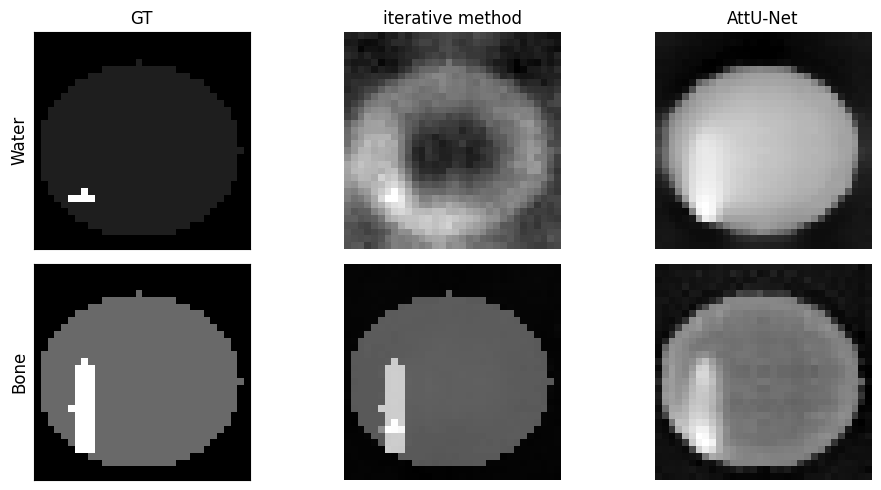
\includegraphics[width=0.7\linewidth]{files/4d5189193864173bd7401583d2dc1609.png}
\caption[]{caption}
\label{wrong}
\end{figure}

One such case is displayed in figure Figure~\ref{wrong} where phantom 17 can be seen, reconstructed using both the iterative algorithm and the AttU-Net model. The GT has both the water and the bone features located in the lower-left quadrant. For the water density image reconstructed using the iterative approach it can be seen there are no recognisable features from the GT present, however there does seem to be a significant lack of water in the center of the image.

The AttU-Net model has, similarly to phantom 2, a relatively constant value throughout the phantom for the water image, while the bone reconstruction does accurately show the bone feature.

\subsection{Attention map}

\begin{figure}[!htbp]
\centering
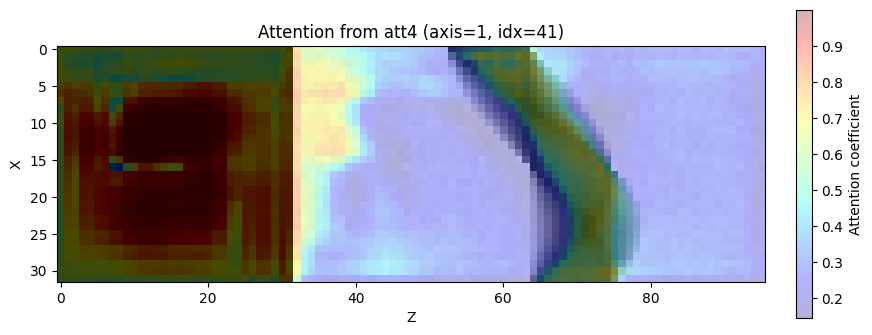
\includegraphics[width=0.7\linewidth]{files/61e001e87d8f0264596b2282806f90e4.png}
\caption[]{An attention map showing how an attention mechanism can be used to have the model focus more on important features, which in this case is the sinogram.}
\label{attention_network}
\end{figure}

Figure~\ref{attention_network} shows an attention map from a AttU-Net model trained on CT scan reconstruction. An attention map has been drawn to illustrate $\alpha_{i}^{l}$ for the first skip-connection. For this specific application it is as expected the attention gate focuses on the lower-intensity parts of the sinogram as these areas provide the most information about the imaged object.

\section{Discussion}

\subsection{Model is only as good as your data}

First, the trained AttU-Net model reconstructed 20 images based on a validation set of phantoms. The first 4 reconstructions of the second phantom are shown in Figure~\ref{bone_recons} where we can see the model recognises features present in the phantom but fails to fully distinguish between bone and water features. Looking at the RMS error over time for the first three phantoms as plotted in (\#reconPhantom), the reconstructions generated using the AttU-Net model have a lower RMS error early on before converging to a higher value than the iterative algorithm.

Looking at the final iterations of the iterative algorithm for the 20 validation phantoms, it can be seem some images do not converge to a visually accurate state as displayed in figure Figure~\ref{wrong}. The iterative algorithm does not always generate reliable results, in this work these unreliable results have been used as training data. This possibly explains why the AttU-Net fails to converge as more iterations are generated, as the network has been trained on data where a subset does not converge either.

The AttU-Net model does recognise features present in the phantom but fails to iteratively get closer to the ground truth. This is apperent from the features present in the reconstructed images of the first iterations shown in Figure~\ref{bone_recons}, and the convergence to a higher RMS error than the iterative aproach for all phantoms shown in Figure~\ref{reconPhantom}. Part of this result can be explained using the common phrase `a model is only as good as the data it gets'.

Looking at the reconstruction results shown in Figure~\ref{wrong}, it is clear the iterative algorithm does not always generate reliable results. Similar images will have been used during training as well, which can negatively impact the training results. For future research it's recommended to only use images reconstructed using the iterative aproach with a rms error smaller than a set threshold to ensure quality of the data.

\subsection{non-machine learning speedup}

Averaging over all 20 reconstructions of the validation set for both the iterativ algorith and the AttU-Net model, an average speedup can be defined as the average time it takes for the iterative aproach to reach the same RMS as the model.

Looking at the reconstruction time, the AttU-Net is more optimised than the iterative algorithm. The AttU-Net makes use of the PyTorch framework which is highly optimised for machine learning tasks. The iterative algorithm has been implemented from scratch and does not include any form of optimisations. For future research it is recommended to also optimise the iterative approach by, for example, performing the matrix multiplications from equation (\ref{projection_eq}) in parallel. This makes for a more accurate comparison of the rms error against time for the two methods.

\subsection{Image size, model size, number of projections}

The current network as defined in the \href{\#}{notebooks}
Currently, it's hard to predict how the running time of the AttU-Net model will grow as the input image grows. The model currently takes 0.5 GB of storage for a 32 x 32 x 32 image. Testing the model for bigger images will require a larger number of projections as well to capture all the image. On top of that the number of channels within the network must increase for each layer to accomodate a larger feature map. To properly compare running times, one must a build model similar to the AtttU-Net model which reconstructs larger images with the same average error. This makes sure no accuracy is lost during comparison.

\subsection{Adding cross attention between spaces}

adding cross attention can more accuratly predict which part of the sinogram attend to which parts of the image. Now two different spaces, image space and projection space, are added into a single matrix. Cross attention might be able to seperate these better.

\subsection{regularisation term}

Looking at the image reconstructed by the AttU-Net model for the bone density seen in Notebook-code, the model could perform better if a regularisation term is added. Look into possibility of performing iterative algorithm after a certain speedup with the proposed model.

\section{Conclusion}

In this work it's been shown that a U-Net model with attention gates in the skip-connections can recognise features present in a phantom but is unable to differentiate between different materials. The AttU-Net model is supposed to gene

\clearpage
\bibliography{main.bib}

\end{document}
